%%%%%%%%%%%%%%%%%%%%%%%%%%%%%%%%%%%%%%%%%%%%%%%%%%%%%%%%%%%%%%%%%%%%%%%%%%%%%%%%%%%%%%%%%%%%%%%%%%%
\chapter{Background} \label{ch:Concepts}

\section{Introduction}
In this chapter we will discuss some important concepts relevant to this dissertation. This include an overview of both \ac{LiDAR} and \ac{FMCW} radar technologies, the components needed to achieve autonomous navigation,  and a quick overview of the \ac{ROS} platform.

\section{\ac{LiDAR} and \ac{FMCW} \ac{radar}}
\subsection{Intro}
In order to do complex tasks and compute different complex algorithms robots require some type of information that relates to its state and environment. This information comes from its sensor sources.
The most typical type of sensors used for perception usually are proximity sensors such as laser range finders (\ac{LiDAR}), sonar or the use of a camera. However robots may have have to deal with a wide variety of changing environments like variation in luminosity, weather conditions, presence of dust and smoke, object proprieties etc... The previous highlighted sensors may show difficulty or be completely ineffective under this conditions.

However the new emerging \ac{mmWave} \ac{FMCW} radar technology with high frequency and bandwidth of 77-81 GHz is now beginning to be suitable for use in robotic applications, and with may provide to be a solution for the previous conditions. In the following  sections we will give a brief overview of current work being done using \ac{LiDAR} and \ac{FMCW} \ac{radar}, how they work, and what limitations each sensor has.

\subsection{LiDAR}

\ac{LiDAR} is a remote sensing technology that tracks the distance of objects. It has been a staple in sensing technology in recent history. It has almost an  unlimited  number of applications \cite{lidar100uses} due to its generation of dense data. Some of the most standing out ones are in autonomous vehicles and robotics:
\subsubsection*{Autonomous Vehicles}

The use of \ac{LiDAR} in autonomous vehicles has been a common trend for a while now. Fig. \ref{fig:lidarcar} ilustrates how multiple of this sensors are used to provide full road environment perception. The insanely accurate depth information combined with a high field of view provided by \ac{LiDAR} enables the development of advanced navigation systems that are able to perform self-driving.
 
 
\begin{figure}[h] 
\centerline{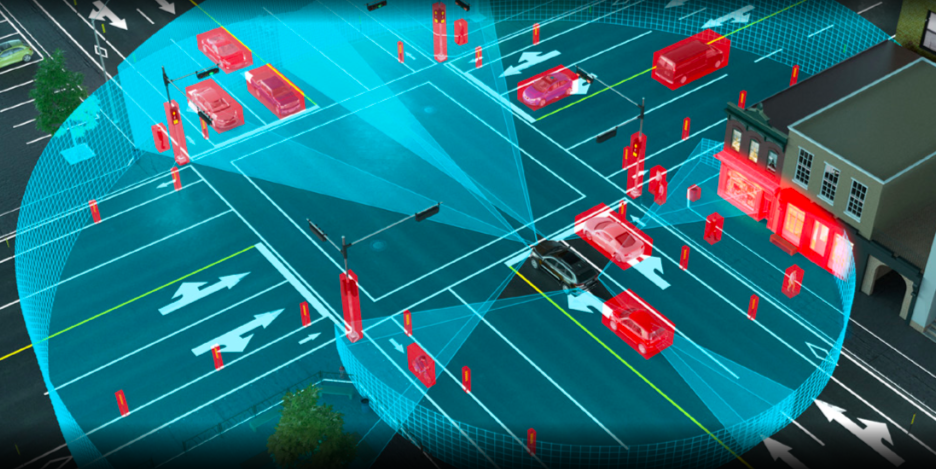
\includegraphics [width=0.7 \textwidth]{imgs/chapter2/lidarcar.png}}
\caption{Example of \ac{LiDAR} technology being used for road perception \cite{lidarcar}}
\label{fig:lidarcar}
\end{figure}

Some application examples of this include \cite{lidarperception}  where it was implemented a perception system for ground vehicles using segmentation, clustering and tracking techniques.  However, it was noted that it was hard to distinguish between closely separated obstacles adding that a movement detection algorithm should be implemented to solve this problem. 


In \cite{car2dlidar} a low cost solution for object detection, classification and ranging is  proposed by the use of an inexpensive 2D pulsed light \ac{LiDAR}. The system was able to provide reliable detection of 1 meter wide obstacles at distances less than 10 meters.


However there are some concerns about this type of technology. CEO of Tesla, Elon Musk has been very critical of it. Recently, at Tesla’s first Autonomy Day event  he said \textit{"Anyone relying on \ac{LiDAR} is doomed. Doomed!"} \cite{elon}. He believes that cameras, radar and ultrasonic sensors are the future for car visions systems. 
\subsubsection*{Robotics}
\ac{LiDAR} is also one of the major sensory component for robotics (Fig. \ref{fig:robotslidar}). Various robots rely on it for autonomy and navigation.
\begin{figure}[h] 
    \begin{minipage}[b]{.49\linewidth}
        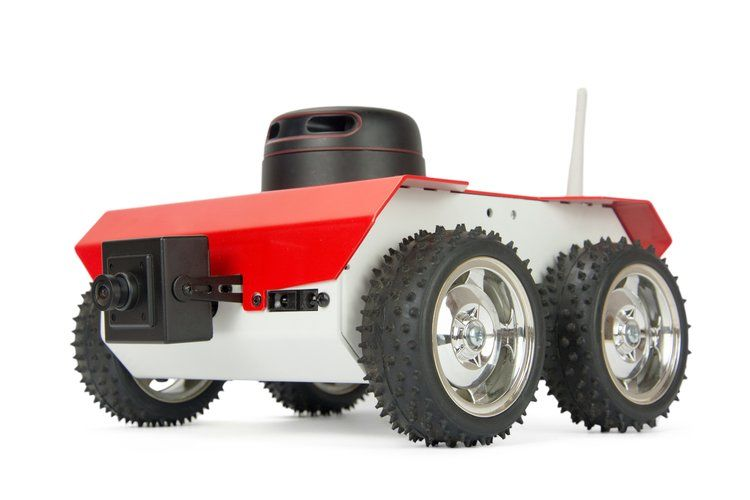
\includegraphics[height=5cm,width=\linewidth]{imgs/chapter2/robot1.jpg}
        \subcaption{ROSbot - Autonomous Robot with Laser scanner RPLiDAR A2 \cite{robot1}}
    \end{minipage}
    \begin{minipage}[b]{.49\linewidth}
        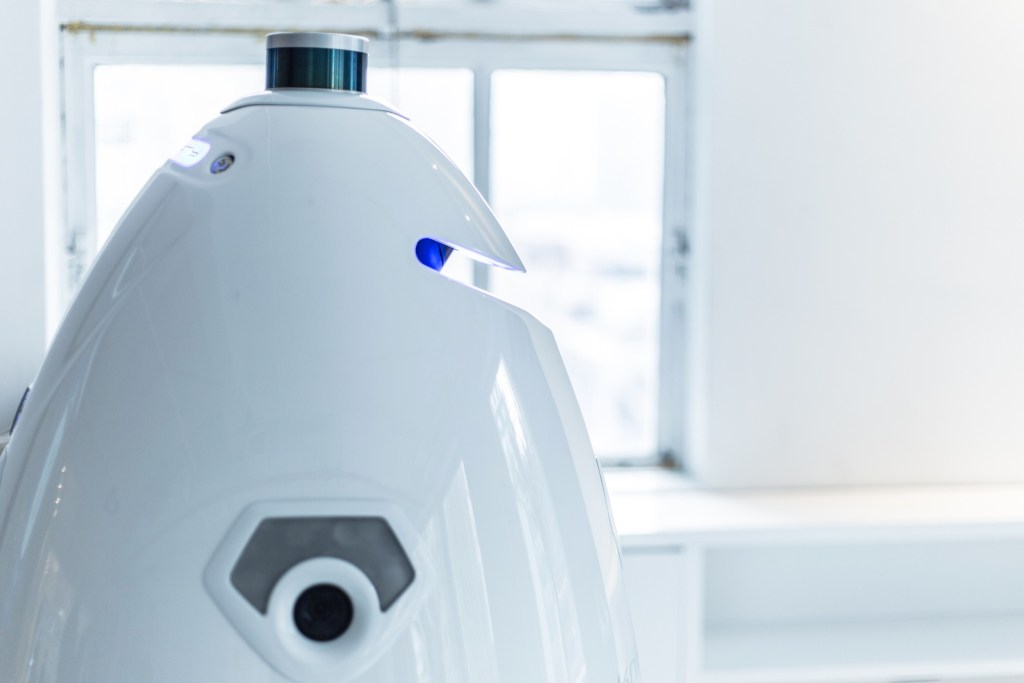
\includegraphics[height=5cm,width=\linewidth]{imgs/chapter2/robot2.jpg}
        \subcaption{Knightscope autonomous security robot with a Velodyne \ac{LiDAR} Puck \cite{robot2}}
    \end{minipage}
    \caption{Different robots using \ac{LiDAR}}
    \label{fig:robotslidar}
\end{figure}


In one of the most popular works with robotic navigation called \textit{"The Office marathon"} \cite{marder2010office}  the PR2 robot was able navigate autonomously for 26.2 miles in an office like environment. During the task, the robot was able to avoid  shelves, tables, chairs and people as well as go
through narrow spaces. The sensor source used in this case was the Hokuyo UTM-30LX Scanning Laser Rangefinder and the navigation system developed is now known as the \ac{ROS} navigation stack. However it was noted that the robot had difficulty detecting low long obstacles.


In a more recent case study in \cite{lidar2019ros} two different systems are proposed for the implementation of an autonomous  mobile robot, both using a 2D \ac{LiDAR} sensor under \ac{ROS}. Various trails in an indoor environment were conducted with both of them and it was concluded that both performed reasonably well but had some difficulty detecting certain types of objects.  

%%ADD ROBOT INDOOR NAVIGATION
\subsubsection{Operating Principle}
The way \ac{LiDAR} technology works is very straightforward, just emit a laser beam and wait for it to bounce back. Based on the proprieties of the reflected signal it can determined the range of the obstacle it hit. By constantly spinning the mirrors at different angles (scanning) we get angle and depth information about the environment  by a  set of points or in other words a pointcloud. There are two main different operating principles to do this, \textbf{Time of Flight} and \textbf{Phase Based} which are described bellow.
\subsubsection*{Time of Flight}
 In this approach a pulse of light is transmitted, when this is done an internal clock is started. The pulse is captured by a photodetector which triggers the clock to stop. Being $\tau$ the time it took for the reflected signal to  comeback and assuming it traveled at approximately the speed of light ($c$) then the distance of the object $d$ is equal to:
\begin{equation}
    d=\frac{\tau c}{2}
\end{equation}
This method produces very accurate results for a wide range but requires high precision clocks. However greater  range capability leads to slower update rates since it has to wait more time for the pulse to comeback.
It is typically not used for robotics since this types of systems have very high cost.
\subsubsection*{Phase Based}
A more affordable approach  is based on modulating the intensity of the laser at a specific frequency. Figure \ref{fig:cwlidar1} showcases the resulting sinusoidal wave that is sent and the respective returned signal. 
\begin{figure}[h] 
\centerline{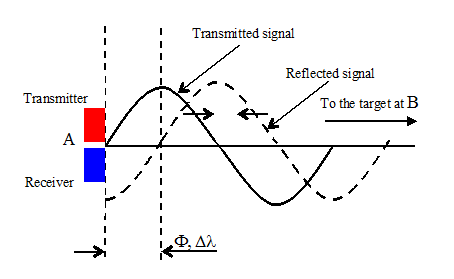
\includegraphics [width=0.7 \textwidth]{imgs/chapter2/cwlidar1.png}}
\caption{Phase comparison method of measuring distance \cite{cwlidar}}
\label{fig:cwlidar1}
\end{figure}

Being $\Phi$ the phase difference between the two and $\lambda_m$ the wavelength of the sinusoid then the distance of the object is given by:
\begin{equation}
    d=\frac{\Phi \lambda_m}{4 \pi}
\end{equation}
This means that the maximum unambiguous distance that can be measured is  $\frac{\lambda_m}{2}$, and its range resolution depends upon the resolution of the phase difference measurement as well as the wavelength used. Almost all robots use this type of \ac{LiDAR} since it is usually cheaper and as a faster update rate.
%difficult to generate continuous wave of high energy

\subsubsection{Limitations}
\ac{LiDAR} technology has some problems associated with it, they are:
\begin{itemize}
\item{High operation costs that limit their use for small applications.}  
\item{Limited detection range compared to radar technology.}  
\item{Sensors are usually bulky and fragile.}  
\item{Direct exposure to sunlight may negatively impact the sensor maximum range and accuracy or even prevent it from functioning completely.} 
\item{Slow measurement rate due to large dataset processing.} 
\item {If it is a 2D-\ac{LiDAR} it only senses using only a single horizontal scanning line}
\end{itemize}
The last item on the list proves to be a significant problem because the sensor has difficulty detecting objects that are above or bellow the height of the sensor (Fig. \ref{fig:2dlidar}). The inability of detecting this type of objects may be crucial for the success rate of the robot being able of doing a certain navigation task safely.
\begin{figure}[ht!]
    \centering
    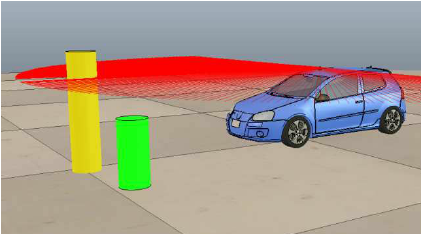
\includegraphics[scale=0.7]{imgs/chapter2/lidar2d.png}
    \caption{Figure illustrating that the 2D \ac{LiDAR} only detects objects in one plane (this plane is usually parallel to the ground (taken from \cite{yalcin2013approaches})}
    \label{fig:2dlidar}
\end{figure}

\subsection{FMCW Radar}
\subsubsection{Intro}
The use of \ac{radar} technology has been around since the 19th century when it was first discovered that radio waves reflected off metallic surfaces, but serious development of this type systems only truly began in the 1930's for military applications \cite{radar_history}. This include the range and angle detection of ship and aircraft engines by measuring incoming signal fluctuations off an oscilloscope. 

Nowadays there are various configuration types of radar systems  \cite{types_radar}, each one providing different types of applications. This usually include air traffic control, remote sensing, ground traffic control, space etc... .  However we will focus on a specific configuration called \ac{MIMO} linear (sawtooth)  \ac{FMCW} radars with  which are  able to measure distance, velocity, and also angular information. 

\subsubsection{Applications}
Multiple works are constantly being done as of right now using this type of sensors. Bellow we showcase some of them.

  \subsubsection*{Pedestrian detection}  
 In \cite{heuel2010pedestrian} three systems are implemented, the first one only using a single radar measurement, the second using multiple, and the final one with additional tracking algorithms. Each system had the objective of distinguishing between people walking, vehicles, and other objects. In the end it was concluded that that \ac{FMCW} \ac{radar} can be used for classification of inroad objects with relatively good precision in all systems.
  
   Another case study is in \cite{knudde2017indoor} where by a processing pipeline the system proposed was able to detect and track people in indoor environments using a 77 GHz FMCW MIMO radar.
   
 \subsubsection*{Localization of Land Vehicles}  
  Vehicle localization is often done by \ac{GPS} accompanied by \ac{RISS}. there are various conditions in which \ac{GPS} signal can not be received correctly. This is often due the land vehicle being in an indoor environment or high rise building blocking the signal. In \cite{abosekeen2018utilizing} it is proposed a radar based \ac{RISS} that not only seeks odometer information but also radar readings. This proved to make the localization system of the vehicle more robust.
  
\subsubsection*{Monitoring of human vital signs}  
Monitoring vital signs of a patient such as the breathing rate or hearth rate may be critical for some patients.
In \cite{alizadeh2019remote} a system for detecting this type of signals using \ac{mmWave} \ac{FMCW} \ac{radar} is proposed. By doing a phase analysis of the \ac{radar} signal it was concluded that the proposed system measurement was in tune with a reference ground truth signal. It was concluded that by increasing the \ac{SNR} of \ac{radar} it could estimate the heartbeat (\ac{ECG}) waveform of multiple targets.

\subsubsection{How it works}
This \ac{FMCW} \ac{mmWave} \ac{MIMO} radar can retrieve range, velocity and angle multiple targets.. The following sections will try explain how to calculate each one of this components.


An \ac{FMCW} radar transmits a signal called a “chirp”. A chirp is a electromagnetic sinusoid whose frequency  increases linearly with time. A chirp is characterized by a start frequency (fc), bandwidth (B) and duration (Tc). The slope (S) of the chirp is the rate at which the frequency of the chirp increases and is given by:
\begin{equation}
    S=\frac{B}{T_c}
\end{equation}
%% put A t and f t plot
Figure \ref{fig:At} shows the plot of the amplitude in function of time for the described chirp. As we can see the frequency of the sinusoid is increased with time. Another way of illustrating the chirp is by its frequency versus time plot (Fig. \ref{fig:At}). The latter version is often preferred due to being more intuitive.

\begin{figure}[h] 
    \begin{minipage}[b]{.49\linewidth}
        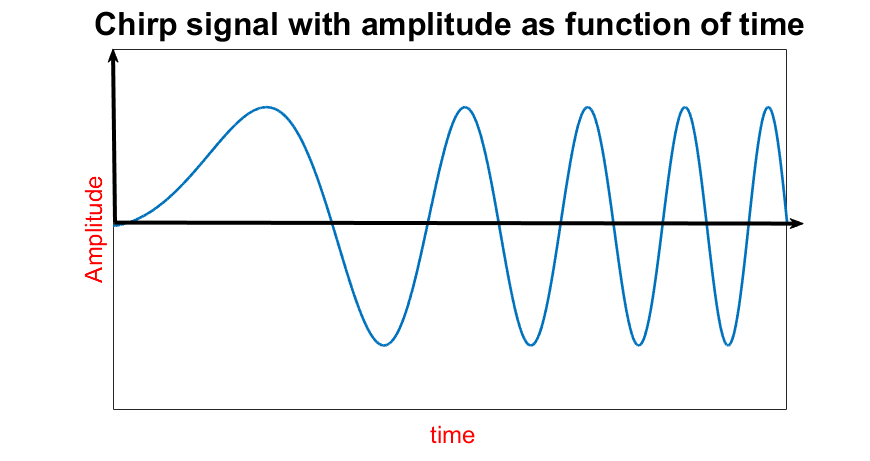
\includegraphics[height=5cm,width=\linewidth]{imgs/chapter2/chirpAt.png}
        \subcaption{Chirp signal with amplitude as function of time}
        \label{fig:At}
    \end{minipage}
    \begin{minipage}[b]{.49\linewidth}
        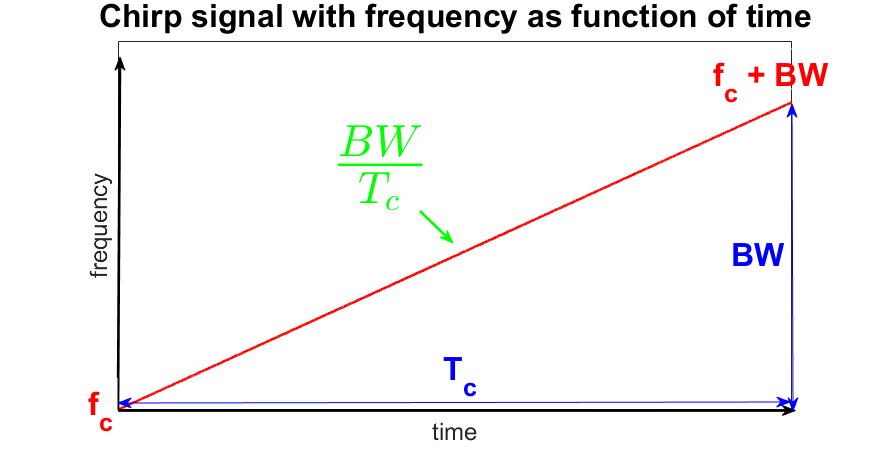
\includegraphics[height=5cm,width=\linewidth]{imgs/chapter2/chirpFt.png}
        \subcaption{Chirp signal with frequency as function of time}
        \label{fig:Ft}
    \end{minipage}
    \caption{Different ways of displaying a chirp}
    \label{fig:robotslidar}
\end{figure}

%%PUT SOME TEXT


Object detection follows this steps:
\begin{enumerate}
    \item The chirp is transmitted by the TX antenna
    \item The chirp is reflected off an object and the reflected chirp is received at the RX antenna
    \item The RX signal and TX signal are ‘mixed’ and the resulting signal is called an ‘IF signal’
\end{enumerate}
Figure \ref{fig:if} shows graphically how the IF signal is generated through both the RX and TX signal for one target detection.
\begin{figure}[h] 
\centerline{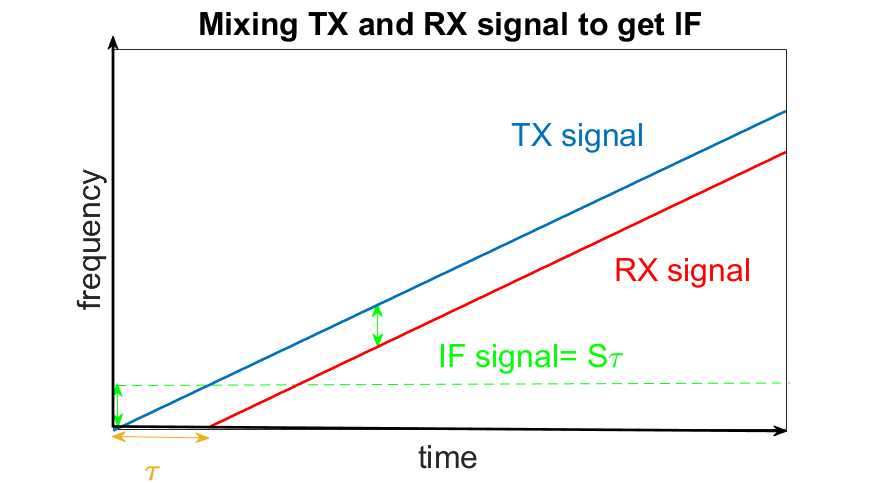
\includegraphics [width=0.8 \textwidth]{imgs/chapter2/IFsignal.png}}
\caption{IF signal creation to retrieve range information of the target}
\label{fig:if}
\end{figure}

%%PUT IMAGE
%%%When the transmitted chirp encounters an object it will reflect back to the radar and will be captured by the RX antenna.
\subsubsection*{range Detection}
The RX signal is a sum of delayed versions of the TX signal. This means that the resulting \ac{IF} signal will be a combination of sinusoids. Each of this correspond to a reflection of an object. For object $i$ the corresponding frequency $f_i$ is equal to:
\begin{equation}
    f_i=S\tau_i
\end{equation}
Where $\tau_i$ is equal to the round trip delay of the wave and is equal to:
\begin{equation}
    \tau_i=\frac{2d_i}{c}
\end{equation}
Where $d_i$ corresponds to the distance of the object to the radar and $c$ the speed of light.
%% PUT image
Putting this together the distance to the object $i$ is given by:
\begin{equation}
    d_i=\frac{f_ic}{2S}
\end{equation}


 So to determine the range of all objects detected we only need to find the according frequency components in the \ac{IF} signal. To do this the analog signal is first sent to an \ac{ADC} and with the resulting digital output the \ac{FFT} is computed by a \ac{DSP}. Each peak in the \ac{FFT} that meets a certain \ac{SNR} threshold corresponds to a different range detection. 
 
 However since the \ac{ADC} has a limited sampling rate, the valid range of frequencies in the \ac{FFT} is also limited, this means there is a maximum amount of range the radar can detect.
The range resolution is also finite since the \ac{FFT} has a limited amount of samples. In short, the higher the bandwidth of the chirp the better resolution we get.
 
\subsection*{velocity Detection}
This type of radar also provides an estimate on the radial velocity for each detected range. To do this more than one chirp is needed. For a set of N chirps we call a frame. The radar constantly sends this frames, each one corresponding to an observation. Since the time between frames is so low the corresponding range (or first) \ac{FFT}s will have  identically located peaks (the same obstacle is in the same range for all chirps in a frame) . However this set of peaks have different phases between each other. By calculating a second \ac{FFT} (Doppler-FFT) of this vector of phases we can extrapolate a set of relative radial velocities  for each range detection. In the end we get a matrix that relates radial velocity and range. 
Figure \ref{fig:matrix} illustrates this process.
\begin{figure}[h] 
\centerline{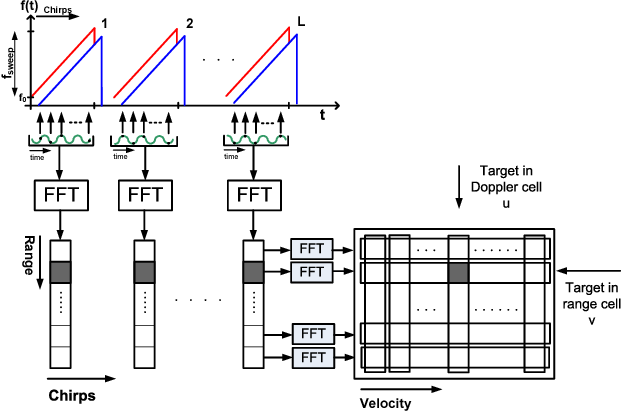
\includegraphics [width=0.8 \textwidth]{imgs/chapter2/dopplerFFT2.png}}
\caption{(taken form \cite{schroeder2010x})}
\label{fig:matrix}
\end{figure}
\subsection*{angle Detection}
Finally to discover the angle for each target we need more than one receiver antennas.This is where the \ac{MIMO} configuration comes in. Figure \ref{fig:angle} shows that for the same target the distance for the two antennas is different.  This difference makes it so for the same peak in the range \ac{FFT} and doppler \ac{FFT} the phase of the received signal is different in the two antennas. If we know this phase difference we can retrieve angle of arrival of the target. 
\begin{figure}[h] 
\centerline{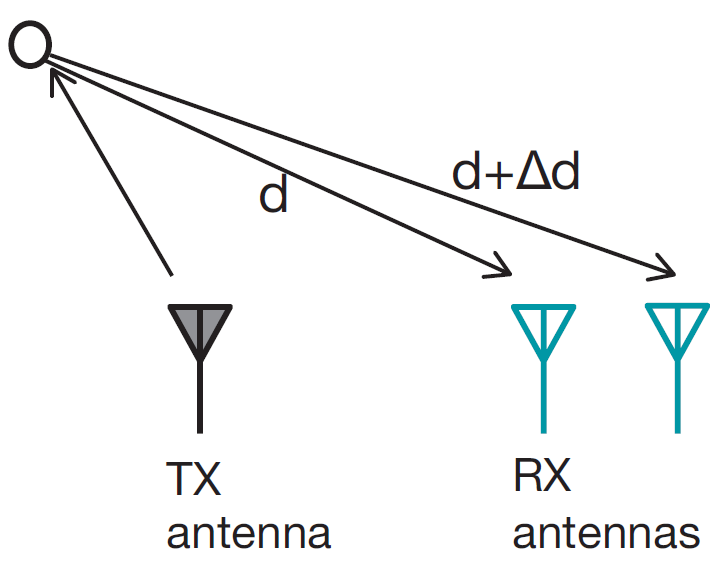
\includegraphics [width=0.5 \textwidth]{imgs/chapter2/angle.png}}
\caption{(taken form \cite{iovescu2017fundamentals})}
\label{fig:angle}
\end{figure}
The phase difference $\Delta \phi$ is given by:
\begin{equation}
    \Delta \phi=\frac{2 \pi \Delta d}{\lambda}
\end{equation}
By basic geometry we know that $\Delta d =L sin(\theta)$ where $L$ is the distance between the antennas and $\theta$ is the angle of arrival. 

\begin{equation}
    \Delta \phi=\frac{2 \pi L sin(\theta)}{\lambda}
\end{equation}
Then the angle of arrival is finnaly given by:
\begin{equation}
    \theta = sin^{-1}(\frac{\lambda \Delta \phi}{2 \pi L})
\end{equation}
The above equation makes it possible to estimate the angle of arrival. But since $\phi$ has a non linear dependency of $\sin(\theta)$ then the angle of arrival accuracy depends on the angle of arrival. The closer it is to $0º$ the more accurate is the result.

 
\subsubsection{Limitations}
\ac{FMCW} {radar} technology has some problems associated with it, they are:
\begin{itemize}
\item{Limited range and angular resolution when compared to \ac{LiDAR} which make difficulty to distinguish between two close targets}  
\item{Low pointcloud density}  
\item{RADAR cannot provide the exact geometry of an object because of the longer wavelength}  
\item{Can have intermodulation products that result in ghost objects} 
\end{itemize}

%GIVE OVERVIEW OF THE CURRENT SENSORS LEADING INDOOR NAVIGATION.

\section {Navigation Concepts}
There are four main problems associated with robotic autonomous navigation. They are Cognitive Mapping, Localization, Path Planning and Motion Control \cite{baranov2014}.  various algorithms have been developed over the years to combat this problems. In the sections bellow we give a brief overview of the more popular solutions.

\subsection{Mapping}

Creating a map in ROS is typically done by using an improved version of  Rao-Blackwellized particle filters such as the ones described in \cite{grisetti2007improved}. This approach has proven to be an effective way to solve the \ac{SLAM} problem and will be used later on in this work to produce a valid map of our indoor environment.
%gmapping, slam, eurico LASER
\subsection{Localization}
With the grid map built we now need to estimate the robot's position in said map. 
An easy solution to this problem is relying on the robot's odometry information inferred by the robot's encoders and inertial sensors such as accelerometers and gyroscopes. This kind of dead reckoning is an easy and low cost solution for the localization problem. However since the sensor data is integrated over time, this leads to the accumulation of errors which make this approach not feasible for long navigation tasks. 
To fix this issue various algorithms were developed being the most popular ones based on particle filters.
The \ac{AMCL} algorithm  is the standard choice in this case. It takes into account a group of particles, each one corresponding to a certain robot state (position and orientation in this case). As the robot moves the least probable states are filtered out and  the particles should over time converge on the actual position of the robot.  
\subsection{Path Planning}
Assuming the robot can localize itself on the map with a reasonable error we can start sending navigation goals to the robot. To reach the goal the robot must be able to find a path that optimizes the travel distance while avoiding obstacles. The outputted plan can vary depending on the algorithm used. In our case we will use the well known dijaktra algorithm.
\subsection{Motion Control}
After the optimal plan is computed the final step is to determine the best velocity command that will be sent to the base.  The ROS navigation system follows a similar approach to the one used in \cite{gerkey2008planning}. A set of velocities are simulated during a given set of time and the corresponding predicted trajectories are  computed. For each trajectory it is calculated a determined cost given by a cost function  taking into account 

\section {ROS}
Creating software for robotic applications is not an easy task to do from scratch. It usually involves very complex code to achieve even the simplest applications due to the wide variety of hardware and data that robots rely on. \ac{ROS} fixes this issue by being a general purpose framework for robotics. Despite its name, it is not an operating system, it is more a kind of middleware, in other words it  handles communication between programs in a distributed system. You can either construct one program that does all the computation needed in your application or you can have sub programs with each one having a specific functionality, the latter is often preferred.

\ac{ROS} provides hardware abstraction, device drivers, tools for introspection, message-passing and more. Also it is open source which means we can use them for virtually any means which we deem necessary for the development of our application, for example adapting pre established code for a specific case. This greatly facilitates the entrance of new developers to learn and do research in this field.
\subsection{ROS architecture}
The \ac{ROS}  architecture is based on a peer to peer network between processes usually referred to as \textit{Computation Graph}. This structure is comprised by different concepts that we define bellow:
\begin{itemize}
\item \textbf{Nodes} - A node can be defined as a process or piece of software  that performs some type of computation. In \ac{ROS}, for a given application there are typically alot of nodes running in parallel that pass information between each other. For example  controlling the robot movement given the input image of a camera requires a node to act as a driver between the camera firmware and the ROS environment. Then there could be a node that processes the image further using ROS pre established software and finally given the processed information a different node will calculate the velocity of the robot and transmit them to the wheels of the robot. 
\item \textbf{Messages} - \ac{ROS} uses predefined data structures  called messages to interpret information. This makes it so \ac{ROS} tools to generate the appropriate source code in the selected language (C++ or phyton in this case). Each message can be broke down into more messages and so one and so forth until we arrive at the primitive data types of the given programming language. Nodes communicate by publishing or subscribing  to topics using this messages and in the end we get a fully alive system that performs some type of application we want. 
ROS predefined data type used to communicate between nodes.
\item \textbf{Topics} - Nodes can send messages by publishing to a topic or receive them by subscribing to a topic. For example a node can be subscribed a raw velocity message and then after some data processing publish a smoothed version of it into another topic.  
\item \textbf{Master} - Provides registration and naming for each node (helps nodes find each other). It is also responsible for organizing communication between nodes. Finnaly it also provides the \textbf{Parameter Server} (described bellow).
% V
\item \textbf{rosout} - This can be viewed as the ROS equivalent of stdout. This tool acts as a log reporting mechanism which is useful when debugging large amounts of code.
\item \textbf{Paramater Server} -In this server \ac{ROS} tracks different paramater values defined by the running application. It is useful for modifying different parameters dynamically without having to restart the application.
%X
\end{itemize}


%%REVER ISTO

Figure \ref{fig:rosgraph} gives a brief overview of how each of this concepts are put together and  generate the in ROS  computation system.

\begin{figure}[h] 
\centerline{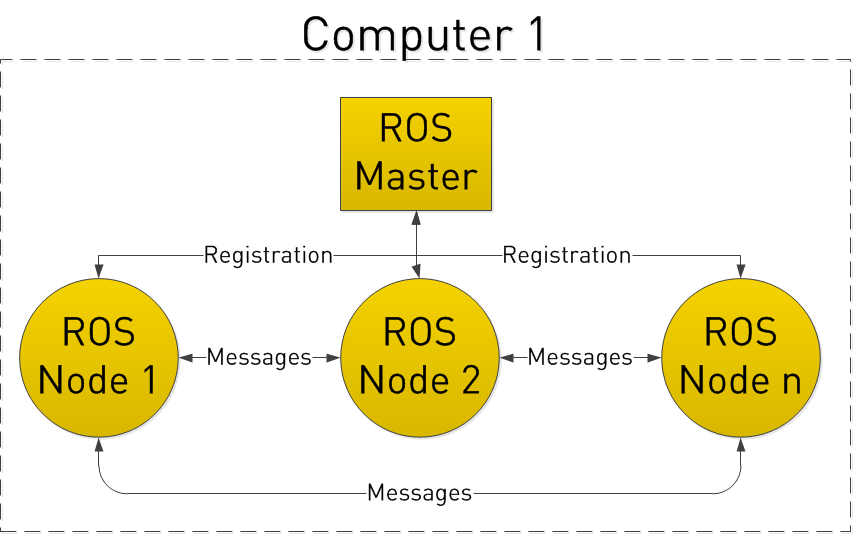
\includegraphics [width=0.5 \textwidth]{imgs/chapter2/rosgraph.png}}
\caption{ROS communication architecture overview \cite{rosbasics}}
\label{fig:rosgraph}
\end{figure}


